\documentclass[letterpaper,twocolumn,9pt]{article}
\usepackage{usenix,epsfig,endnotes,url,verbatim,array,fancyvrb,graphicx,grffile}

% For representing code in paragraphs.
\newcommand{\code}[1]{\texttt{#1}}

\begin{document}

\title{\Large \bf Web-based Data Analytics in Haskell}

%don't want date printed
\date{}
%make title bold and 14 pt font (Latex default is non-bold, 16 pt)

%for single author (just remove % characters)
\author{
{\rm Drew Haven, Eric Stratmann}\\
\{drew.haven, eric.stratmann\}@gmail.com
% copy the following lines to add more authors
% \and
% {\rm Name}\\
%Name Institution
} % end author

\maketitle


\begin{abstract}
Many people are interested in statistics, but providing an easy to use Website to analyze statistics can be difficult. We wanted to make it simple to create Websites to analyze arbitrary data. Our project explored data analytics using the Haskell Web framework, Yesod, using it to write a proof-of-concept site that analyzes information from the popular on-line game League of Legends. The Website allows users to lookup a variety of statistics and perform queries on the data while presenting the results in a graphical format.
\end{abstract}

\section{Introduction}

Analyzing statistics can be rewarding and insightful, but without an easy way to analyze new datasets doing so can be difficult. Statistics are useful in a variety of fields. For example, although no knowledge of statistics is required to play baseball, many fans of the sport love to analyze baseball statistics. Since baseball is popular there are many Websites to analyze baseball data, but what about less popular data? Creating a site to analyze new sets of data can be time consuming. Although there are many existing statistics packages, they are often hard to use and do not provide a Website for others to browse. Users are often left managing large spreadsheets to keep track of their data.

 While the data being analyzed across different datasets may differ considerably, the sorts of queries that people are interested in are often similar. People would like to correlate different variables, filter on certain conditions, and retrieve subsets of the data. They would like to do calculations on the data (sums, averages, counts) and display this information in tables or charts. We wanted to see if we could provide this functionality in a generic way for generic datasets. 

We created a demo application using data from the on-line video game, League of Legends~\cite{lol}. League of Legends is a competitive Real Time Strategy games where teams of five play against each other. The site allows users to view player information and analyze various gameplay statistics. Users can look at their own data to learn about their behavior in the game or look at more general data to see trends in gameplay. Besides creating the site itself, we also wrote software to parse and upload League of Legends data. 

Our aim in creating this application was to determine what sort of database interface would help us write this Website, as well as to evaluate Haskell's viability for Web application development. We chose to use the Yesod framework, which seemed to be the most mature Haskell Web framework. For our backend, we used the MongoDB\cite{mongo} database, and wrote code to automatically generate MongoDB queries based on columns defined on our dataset. Our paper discusses the issues, limitations, and advantages of our approach.

The rest of the paper is organized as follows. Section \ref{sec:background} provides some background on technologies we depended on for our project. We discuss our results in section \ref{results}. Section \ref{site} looks at our example site. In section \ref{future} we discuss possible future directions of our work. Finally, section \ref{conclusion} concludes.

\section{Background}
\label{sec:background}

\subsection{Yesod}

Yesod~\cite{yesod} is one of several Web frameworks written in Haskell. Like many other frameworks, Yesod uses both MVC and RESTful URLs, making it in some ways similar to more traditional frameworks. Being written in Haskell, however, Yesod allows developers to take advantage of unique Haskell features.

To write controllers, developers can use Yesod's monads, \code{Handler} and \code{Widget}. These build up HTML, CSS, and Javascript, and allow modifying and reading HTTP headers. These monads are instances of MonadIO which allows controller pages to execute arbitrary IO actions as well as generating the page. See Figure \ref{controller} for an example controller. This example queries a lists of games and paginates them into groups of 10. It then renders the page and includes a list template which shows information about each game. Part of this page can be seen in Figure \ref{list}.

Like most other frameworks, Yesod provides templates to make writing HTML, CSS, and JavaScript easier. The templates provide basic variable substitution and control statements, as well as supports for simplified syntax. See Figure \ref{hamlet} for an example of Hamlet, Yesod's HTML templating system, which is used in the controller in Figure \ref{controller}. The template resembles HTML but clearly is not HTML. Closing tags are not specified, Haskell functions are called, other templates are included, and static routes are used to generate URLs.

Yesod uses Haskell's types to provide functionality that is often impossible in other languages. Type safety helps prevent many security vulnerabilities and broken URLs. For example, since URLs are represnted by a special type in Yesod, it is impossible to refer to a URL which does not exist because this would be a type violation. Type inference allows more concise code by automatically detecting what model the developer is querying, as in Figure \ref{controller}. Yesod automatically detects that we want a list of games because how the \code{games} variable is later used.


\begin{figure}[]
\footnotesize{
\begin{verbatim}
getGameIndexR :: Handler RepHtml
getGameIndexR = do
  (games, opts) <- paginateSelectList 10 [] []
  defaultLayout $ do
    let list = $(widgetFile "game/list")
    setTitle "Game Index"
    $(widgetFile "game/index")
\end{verbatim}
}
    \caption{Sample Yesod Controller}
    \label{controller}
\end{figure}

\begin{figure}[]
\footnotesize{
\begin{verbatim}
^{pager opts}

<table.game-list>
<thead>
  <tr>
    <th>
      Teams
    <th>
      Queue
    <th>
      Date Added
<tbody>
  $forall game <- games
    <tr data-href=@{GameViewR (fst game)}>
      <td.champs>
        ^{portraits champions (snd game)}
      <td.queueType>
        #{gsqueueType (gameGameStats (snd game))}
      <td.created>
        #{gameFormattedCreateTime (snd game)}
\end{verbatim}
}
    \caption{Sample Hamlet File}
    \label{hamlet}
\end{figure}

\subsection{Persistent}

Persistent\cite{persistent} is a library developed for Yesod to facilitate data access.  It attempts to make data access type safe, concise, declarative and independent of the underlying data store.  It uses a mixture of typeclasses to achieve this, as well as various language extensions to make some of tricks possible.  The three major pieces of the puzzle are the type classes \code{PersistBackend b m}, \code{PersistField val}, and \code{PersistEntity val}.

The core of Persistent is the \code{Persistbackend b m} typeclass, which defines the basic operations on the database such as \code{insert}, \code{update}, \code{delete}, and \code{get}.  An interesting point is it encodes the backend type in the \code{b} parameter, but also specifies the constraints \code{Monad m}, \code{Monad (b m)}, \code{MonadIO m} and \code{MonadIO (b m)}.  This forces the backend type to provide the mechanism for accessing IO to interface with the database without making any specific statements about how or where \code{PersistBackend} instances can be used, as they all return values in the \code{b m} monad.

Persistent deals with data by having a restricted set of types that it uses internally to interface with the database, the \code{PersistValue} type.  These types closely resemble JSON or BSON types.  They include a few primatives, null, and the two collection types \code{PersistList [PersistValue]} and \code{PersistMap [(Text, PersistValue)]}.  The library ensures that the backend can store values of these types which decouples the application data types and the database's internal representation.

Any datatype that can be stored as a database column needs to be an instance of the \code{PersistField} typeclass.  This typeclass handles the marshalling to and from \code{PersistValue}s.  The close resemblance of \code{PersistValue} to JSON types, specifically \code{Data.Aeson.Value}, allowed us to write code to do an instance of \code{PersistField} for \code{Data.Aeson.Value}, and from that we could utilize the same \code{FromJSON} and \code{ToJSON} instances we wrote for the parsing code to implement a \code{PersistField GameType} instance that we could use to store the game statistics data in the database.  The library understands how to represent \code{PersistValue}s in MongoDB in a way that preserves their structure, which gave us the ability to do deep inspection of the data in the database, which was essential for our query filters and map reduce code.

The final piece of the puzzle is the \code{PersistEntity val} typeclass, which is the one we worked with the most.  This typeclass defines the code for converting a top-level data type to or from column data, the columns present on the data type and unique key constraints.  The most interesting part was the column definitions. These are defined through the \code{EntityField} data type, a type family parameterized by the type \code{val} and the column data type.  \code{TypeFamilies} is an extension that is not commonly used, but is used well in this context.  In this case it is used to allow different constructors of the datatype to take on different types.  This is one of the more interesting examples of how Yesod uses Haskell language features to ensure type safety.  See Figure \ref{EntityField} for an example definition. Note that only \code{GameCreated} and \code{GameGameStats} represent first-level data columns and the others inspect sub-objects.

When put together these components create a declarative way to define data and queries.  Much of the definition can be done through Template Haskell functions, such as \code{derivePersistField} or \code{mkPersist}.  These will define the datatypes and their instances for most common cases.  We wanted to define query columns that inspect the data more deeply than the defaults allow, necessitating writing our own \code{PersistEntity} definitions.  It was surprisingly easy to add additional columns, however the details of how Persistent builds queries restricted them to simple column comparisons in MongoDB. Multi-column functions may be possible in SQL.

Filters are created through comparison functions, which are analogs for familiar comparison functions, such as less-than, equals and set membership.  They are defined by the \code{PersistFilter} data type, and Yesod provides more convenient creation functions such as \code{<.} and \code{==.}.  The filters also ensure type-safety of the comparison (Figure \ref{Filter}).  Note the Rank2Type for \code{typ} which enforces a match between the value and the field's type.  Also note that \code{v} represents the model type, which ensures all filters correspond to columns on the same data type.

Select queries naturally follow from their filters, which encode almost all information needed to make the query.  The select only requires a few additional options such as limits and offsets before it can be executed.

Persistent is a very elegant system for database access, and was a pleasure to work with on this project.  It makes a few assumptions about the data to enable its elegance.  Examples include an inability to model relational data and a restricted set of operations.  Current work on Persistent is attempting to address this by splitting the backend from the query interface so more complex queries can be executed on backends that support them.

\begin{figure}[]
\scriptsize{
\begin{verbatim}
data EntityField (GameGeneric backend) typ
   = typ ~ (Key backend (GameGeneric backend)) => GameId
   | typ ~ UTCTime   => GameCreated
   | typ ~ Bool      => GameRanked
   | typ ~ Int       => GameGameId
   | typ ~ Int       => GameLength
   | typ ~ GameStats => GameGameStats
   | typ ~ Text      => GameTeamPlayerSummoner Text
   | typ ~ Text      => GameOtherTeamPlayerSummoner Text
\end{verbatim}
}
    \caption{EntityField declarations for GameGeneric backend}
    \label{EntityField}
\end{figure}

\begin{figure}[]
\footnotesize{
\begin{verbatim}
data Filter v = forall typ . PersistField typ =>
    Filter { filterField :: EntityField v typ
           , filterValue :: Either typ [typ]
           , filterFilter :: PersistFilter
           }
    | FilterAnd [Filter v]
    | FilterOr [Filter v]
\end{verbatim}
}
    \caption{Filter typeclass}
    \label{Filter}
\end{figure}

\subsection{MongoDB}

Our backend used MongoDB~\cite{mongo}, a documented-oriented database. MongoDB stores data in BSON, a binary-encoded serialization of JSON-like documents, with a few extenstions for additional data types.  The MongoDB query system has two parts.  A simple query system supports for operations analogous to non-relational SQL statements; this is how all basic CRUD operations are performed.  The second query system implements map-reduce.  The map-reduce system uses JavaScript functions to run queries across documents and sharded databases.  MongoDB is schemaless in that the documents have no defined structure or types.  This places the burden on the programmer to ensure data is consistent and well-formed.

\subsection{League of Legends}

League of Legends~\cite{lol} is an on-line real-time strategy game. Although the details are not important since we could have chosen any other dataset to analyze, we provide a quick introduction of the important concepts to put the examples into context. Players (also known as summoners) fight in teams of five against each other using characters known as Champions. The object of the game is to advance to and destroy the other side's base. Players can advance towards this objective by killing other players and completing secondary objectives which they use to gain additional power and gold which is used to purchase upgrades. People are interested in different statistics of summoners and champions, such as their kill and death rates, total gold gained and towers destroyed.

Particularly interesting statistics could arise from comparisons across many players.  For example, the number of secondary objectives completed compared to the average match-making rating of the team, or how secondary objectives impact game length.

\section{Results}
\label{results}

\subsection{Data backend}

The game statistics are represented by a small collection of data types, the major ones being \code{GameStats} and \code{PlayerStats}.  In short, a game is represented by \code{GameStats} which contains game-wide information such as the game length and a field for each team which contains a map from player name to \code{PlayerStats}, which in turn contain individual player information and a \code{Map Text Int} which contains the various additional statistics for the player.  Data is stored in MongoDB and represented fairly close to the original data format.  This is conveniently achieved by using the \code{FromJSON} and \code{ToJSON} instances defined for the original parser.  As the project progressed we altered the data format by performing some transformations on the raw data to remove unnecessary data layers and provide more convenient indexing, this caused the data parsing for raw data and database data to diverge.  We wrote a simple instance of \code{PersistField} for \code{Data.Aeson.Value} and some TemplateHaskell functions to generate the instances.  Basic queries on the data use this interface.

The largest single portion of our Yesod code was written for our map-reduce query interface.  The interface is modeled on Persistent, and is designed to be an alternate query interface.  One major difference is that we want the map-reduce queries to return semi-arbitrary data with respect to the underlying data model, so we cannot return a clear type.  For example, one column that might be requested could be an average of many \code{Int} columns which is represented as a \code{Float}.  Since the number of potential columns is infinite we rely on the programmer to specify them.  Queries also need to be dynamically definable so that users can specify what data they want to access.  We compromised by returning the opaque \code{Value} type, which corresponds to BSON values, and provided a casting operation to safely coerce the value to the correct type.  This puts a burden on the programmer to keep track of which columns are which, but it was deemed acceptable for the prototype.

The query API essentially comes down to two pieces (Figure \ref{mrapi}).  The \code{mapReduce} function is similar to the \code{selectList} function of Persistent.  The \code{Queryable} typeclass (Figure \ref{queryable}) defines the functions for transforming columns into filters and map-reduce code.  The goal is to make it easy to define new columns on whatever your data might be.  To achieve this, most of the functions in \code{Queryable} have default implementations and there is a suite of helper functions which work with the default implementations to limit the amount that needs to be explicitly stated. For example, \code{simpleMap} takes a MongoDB selector fragment and produces the proper code to be inserted into the default map function to extract that item.  There is also an implicit \code{\_count} column which stores the number of documents contributing to the data which is used for building averages.

The implementation allows the JavaScript to be arbitrary, through \code{queryMapFunc}, \code{queryReduceFunc} and \code{queryFinalizeFunc}.  We created a default form which we used in our project while providing the ability to define arbitrary code.  The limits what we were able to do with the system, but constrained the problem space so we could more efficiently implement.  The map step extracts the key with \code{queryKeyCode}, then for each column it runs \code{queryMapCode} which adds the value to the result object which is then emitted with the key.  The reduce code merges two records by iterating over every column and using the corresponding code which can be defined through \code{simpleReduce} by providing just an operator.  The finalize step is run after all the reductions have been performed, and also iterates over all the columns; there are simple helper functions for either totals or averages.  The filtering function works very similarly to Persistent's filters.

The advantage of this interface is that control of the columns is in the hands of the programmer and can theoretically be anything the user could write in a direct MongoDB call, and once written they can be composed, combined, and reused easily.  The queries are also declarative and type-safe, preventing the programmer from mixing columns for different models or providing the wrong type to a filter.

There are three major drawbacks.  The first is that the user has to directly specify JavaScript which is error prone and breaks the abstraction provided by Persistent; the helper functions alleviated some of this, but even for our simple queries we were unable to avoid writing JavaScript expressions.  There may be a way around this, but we were unable to find one that could be implemented in our time constraints.  The second drawback is that each new column may require defining a pattern-match in many functions to deal with the new case; this depends on how complex the JavaScript is and can be fixed by defining some additional functions to reduce repetition.  The final drawback is that the results are returned as BSON \code{Value}s; requiring the programmer to cast the value to a \code{Maybe typ} through \code{getResultValue :: (Val typ, Queryable model) => QueryColumn model typ -> M.Map Label Value -> Maybe typ}.

\begin{figure*}[t]
\footnotesize{
\begin{verbatim}
mapReduce :: (PersistBackend Action m, Applicative m, Queryable model)
  => QueryColumn model typ                 -- ^ The column to use a key.
  -> [QueryFilter model]                   -- ^ A list of filters.
  -> forall typ0. [QueryColumn model typ0] -- ^ A list of columns to select for the output.
  -> Action m [(Label, M.Map Label Value)]
\end{verbatim}
}
    \caption{Map-Reduce API}
    \label{mrapi}
\end{figure*}

\begin{figure*}[t]
\footnotesize{
\begin{verbatim}
class PersistEntity model => Queryable model where
    -- Column definitions
    data QueryColumn model :: * -> *
    queryColumnName     :: QueryColumn model typ -> UString
    queryFilter         :: QueryColumn model typ -> Value -> Document
    queryKeyCode        :: QueryColumn model typ -> Javascript
    queryMapCode        :: QueryColumn model typ -> Javascript
    queryReduceCode     :: QueryColumn model typ -> Javascript
    queryFinalizeCode   :: QueryColumn model typ -> Javascript
    queryCastResult     :: (Val typ) => QueryColumn model typ -> Value -> Maybe typ
    queryMapFunc        :: QueryColumn model typ -> forall typ0. [QueryColumn model typ0] -> Javascript
    queryReduceFunc     :: forall typ0. [QueryColumn model typ0] -> Javascript
    queryFinalizeFunc   :: forall typ0. [QueryColumn model typ0] -> Javascript
    queryCollection     :: QueryColumn model typ -> UString
\end{verbatim}
}
    \caption{Queryable Typeclass}
    \label{queryable}
\end{figure*}

\subsection{Chart generation}

To help users understand the data they are looking at, our Website renders data using graphical charts, such as bar or line charts. While some data is best presented in tabular form, charts can visually display the relationship of different variables in a way that is easy for people to understand. In particular, we thought viewing a chart would help users view correlations between two different variables. Figure \ref{chart} shows a sample chart.

We used the Flot\cite{flot} JavaScript charting package. Flot charts are generated using JavaScript and displayed on an HTML Canvas element. While we had originally tried generating static charts, that did not give us the same level of functionality as the JavaScript charts. Although we didn't end up using any of this functionality, it would have allowed users to sort charts in the browser, click on different elements of a chart to go to the appropriate page, etc.

While it is possible for developers to manually generate JavaScript to create Flot charts, we created a Haskell API that allows developers to specify their charts in Haskell. The API takes a list of display parameters (such as titles, chart size, orientation, etc.) and a list of data points in the form \code{[(key, value)]}. The chart automatically takes care of including any necessary HTML, JavaScript, and CSS and can simply be included anywhere in the page, using Yesod's Widget monad. Figure \ref{chartcode} shows a controller that uses the chart API. 

\begin{figure}[h]
    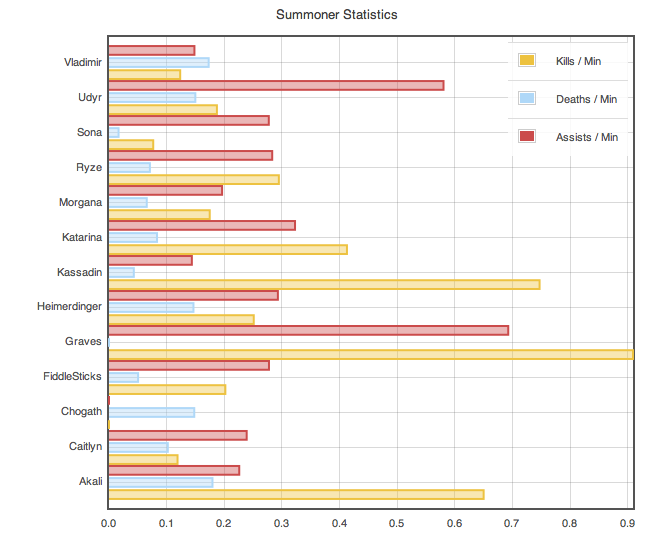
\includegraphics[width=80mm]{imgs/chart.png}
    \caption{Chart}
    \label{chart}
\end{figure}


\begin{figure}[]
\footnotesize{
\begin{verbatim}
summonerChartR :: Handler RepHtml
sumonnerChartR = do
    dataRows <- runDB . runMapReduce $
             buildQuery(QGameChampion summonerName)
        [exists $ QGameSummoner summonerName] columns
    let series = getSeries dataRows

    defaultLayout $ do
        setTitle $ "Stats for " ++ summonerName
        let stats = makeChart summonerChart series
        $(widgetFile "summoner/view")

summonerChart :: Widget
summonerChart =
    setTitles "" "" "Summoner Statistics" $
    setHorizontal True $
    setSize 600 400 $
    barChart
\end{verbatim}
}
    \caption{Controller used to generate a chart}
    \label{chartcode}
\end{figure}

\subsection{League of Legends Logs}

The League of Legends client is written in Adobe Air and runs in the background while games are in progress. Data from the League of Legends game client is dumped to log files.  It has a standardized format that includes fields such as time, log level, and message type, but the most interesting data for our case are the end-of-game stats, which are dumped out by an object dumping routine.  Data in these dumps is very similar to BSON , but structure is based on based on indentation (See Figure \ref{samplelog}).

The first phase of our parsing is to parse object dumps into an \code{ASValue} datatype, which is modeled after \code{Data.Aeson.Value} and described in Figure \ref{asvalue}.  The parsing code is written with Attoparsec, and is straightforward other than the indentation.  Indentation is tracked by wrapping the \code{Parse} monad in a reader transformer that stores the number of spaces on the current indentation.  Every key-value pair of an object or entry in an array first checks for the corresponding level of indentation.  When a new object or array is encountered, the indentation is incremented for the recursive call, and if the indentation fails to parse it simply signifies the end of the object and the \code{many} combinator will return the results parsed so far.

Once the end-of-game log messages have been extracted and the data parsed into \code{ASValue} it can be converted one-to-one into JSON through an appropriate \code{ToJSON} instance.  All our JSON manipulation uses the excellent Aeson library.

Since we want to represent the data internally in a form different from that of the logs we needed to write two functions to parse the JSON; note the awkward \code{ArrayCollection} and \code{ArrayList} objects in the sample that are essentially just a list or vector and the repeated object \#4.  For the database representation we used the TemplateHaskell derivied \code{FromJSON} and \code{ToJSON} instances.  For parsing the raw data we hand-wrote a more complicated parser that does a few minor data transformations along the way, such as indexing some arrays by a key and removing some unnecessary layers of data and duplicate fields.

In the end we can convert logs into \code{ASValue}; \code{ASValue}s to and from \code{Data.Aeson.Value}s; and \code{Data.Aeson.Value}s to and from \code{GameStats}.  In our implementation, the log-parsing client does the conversion from logs to JSON, which is then serialized and uploaded to the server which treats it as the raw JSON form and parses it into \code{GameStats} which it wraps in a \code{Game} model and stores in the database.

\begin{figure}[btp]
\footnotesize{
\begin{verbatim}
body = (com.riotgames.client::EndOfGameStats)#1
  basePoints = 69
  completionBonusPoints = 0
  difficulty = (null)
  elo = 0
  eloChange = 0
  experienceEarned = 0
  gameId = 245368572
  gameLength = 1839
  gameMode = "CLASSIC"
  gameType = "MATCHED_GAME"
  newSpells = (mx.collections::ArrayCollection)#2
    filterFunction = (null)
    length = 0
    list = (mx.collections::ArrayList)#3
      length = 0
      source = (Array)#4
    sort = (null)
    source = (Array)#4
\end{verbatim}
}
    \caption{Sample ActionScript object}
    \label{samplelog}
\end{figure}

\begin{figure}[h]
\footnotesize{
\begin{verbatim}
type Object = M.Map T.Text ASValue

data ASValue =
       ASNumber N.Number
     | ASString T.Text
     | ASBoolean !Bool
     | ASNull
     | ASDate T.Text
     | ASArray !Integer (V.Vector ASValue)
     | ASObject T.Text !Integer Object
     deriving (Show, Eq)
\end{verbatim}
}
    \caption{ActionScript object descriptions}
    \label{asvalue}
\end{figure}

\subsection{League of Legends Log-Upload Client}

The first implementation of the log-parsing client used the parsing code mentioned above and \code{Network.HTTP} to upload the resultant JSON to a server.  This version was very easy to implement.  However, it required the user to run the command from a terminal and provide the directory of the logs as an argument to the program, which is outside the comfort zone of many potential users.

The first revision involved querying the windows registry through the \code{System.Win32} library.  This proved useful, creating a binary that could be double-clicked to perform the uploading, though the output was still displayed in a console.  When distributing the program to alpha testers we found that the registry keys used were not consistent across systems.  This was solved by querying multiple keys until one yielded a result, but even that was insufficient as some users were running the program without having run the installer process and so had no registry keys, and at least one of our alpha testers was also using a non-default directory.

The solution is to prompt the user for the location of the program which forces us to move towards a GUI.  Some brief research suggested wxWidgets as a good cross-platform GUI system.  We set up a system which built a GUI and ran the UI in one thread after doing a directory look up and prompting the user if necessary, then spawned a worker thread to do the parsing and uploading.  The worker thread appended its log messages to a \code{Control.Concurrent.STM.TVar}, which is polled by the GUI to update its display and give the user easier access to error messages and progress information.  We used a \code{ReaderT} wrapper around IO to run actions in a way that they would have access to the log configuration.

The program compiled, but we had difficulty distributing it due to DLL dependencies.  GHC statically links most libraries by default, which was desired for distribution, however when compiling the wx code, it attempts to link many things dynamically including \code{libstdc++}.  Even locating the libraries and placing them in path, other libraries such as \code{libgcc\_s\_dw2-1} were requested by the binary but were not present in the Haskell Platform, wxPack (the wxWidgets distribution), or MinGW (providing gcc).  After going through a few hours of tracking down DLLs, adding static compilation flags, and recompiling, we abandoned the GUI for windows users due to time constraints.

At this time I believe a better approach to a cross platform GUI would be to use another language such as Java which has a track-record of creating cross-platform GUIs. Other GUI libraries for Haskell such as GTK are worth a look to determine if they suffer the same problems as wxWidgets.

\section{League of Legends Site}
\label{site}

We wrote a Website to display League of Legends statistics to determine how well our Peristence integration worked. Although the Website is fairly simple for an analysis site, building the site helped us in developing our query interface. The Website allows users to upload games, view information about games, viwe champion data, and perform analyzis on summoner data. When a game is uploaded, its data is added to the MongoDB database automatically and will be included in all future queries.

Figure \ref{list} shows a list of games, indicating which Champions were used in each match. Figure \ref{chart} shows a sample chart that shows aggregate information about a summoner across all uploaded games the summoner played in, while Figure \ref{stats} shows the same information but in tabular format. The presentation of the results as well as the columns of interest are customizable by the user. In writing these pages, we found that we had to write a lot of code to transform data to and from a variety of formats, but this was fairly easy using Haskell's functional list manipulation. 

Our backend is capable of performing more powerful queries, but we did not have enough time to code more pages to display this functionality. Ideally, users would be able to specify arbitrary queries, giving custom filters, keys, etc. Questions we'd like users to be able to answer include ``How does X correlate to Y for players above a certain skill level?'', ``What is the distribution of game length for different champions?'', or ``Rank all players by the quality of their wins and losses''. 

\begin{figure}[h]
    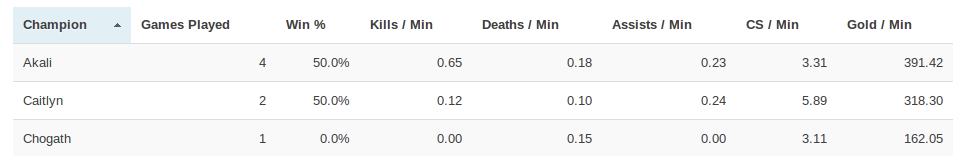
\includegraphics[width=80mm]{imgs/stats.png}
    \caption{Statistics for a summoner}
    \label{stats}
\end{figure}

\begin{figure}[h]
    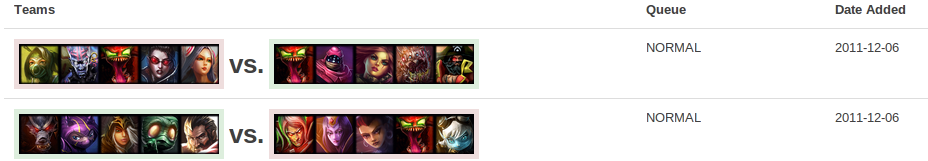
\includegraphics[width=80mm]{imgs/gamelist.png}
    \caption{Game list}
    \label{list}
\end{figure}

\section{Future Work}
\label{future}

Although we are happy with the progress we made on our project, neither the backend nor the Website are production quality.   The project has the potential to be a production-level site, but will require a few more changes.  Specifically, there are some additional features and bugs that need to be fixed in the site itself, it needs to be properly deployed and optimized for performance, and the log-parsing client needs to be polished and finished.

The site itself has enough features to be considered a minimum-viable product, suitable for testing business hypotheses.  There are a few display bugs that simply require a little time to fix.  The more pressing issue is securing permissions of auxiliary data, such as the reference data for Champions and Items.  These are primarily used to commonly configure display names, images, and descriptions of these entities that referenced over many games.  Yesod has support for users and has built-in code for authentication through methods such as the database, Facebook, and Google.  User accounts and permissions were outside the scope and focus of this project.

Yesod does attempt to optimize for performance.  It chose to use the Warp WAI server and Blaze HTML for their speed.  It has made some conscious trade-offs though, such as not optimizing static file handling as that is reasoned to be better achieved through offloading it to an external server such as Apache or Nginx.  These are minor considerations of the specific deployment.  The largest issue is the performance of our code.  Passing our data through an intermediary JSON representation on every save or load may be $O(n)$, but it may add unnecessary overhead.  Our map-reduce framework does not take into account any of the performance peculiarities of MongoDB and was not tested on a sufficiently large dataset for performance issues to manifest.  Yesod's non-relational setup may introduce additional considerations related to the number of queries made to the database, but these were also not tested on a large enough dataset for those latencies to manifest visibly.  In a production deployment of the site, all of these issues would need to be investigated.

Yesod is not finished.  The development team is working towards a 1.0 release, and until then has been updating the interface to accommodate new use cases.  One feature in the development branch that would be beneficial to us is that Persistent has worked to separate the backend and the querying interface, better supporting alternate query interfaces such as our map-reduce interface.  We plan to continue to work with the Yesod development team in the future.

\section{Conclusion}
\label{conclusion}

We had mixed feelings about working with Yesod. Although the framework takes advantage of several Haskell features, the framework is not as mature as those available for other languages. For example, there was little documentation except for the most basic features. This is not too surprising since Yesod is less than two years old and has only a few core developers.  However, we were able to accomplish many of the things we would expect in a modern web framework and Yesod has a lot of potential due to the conciseness and expressiveness of Haskell.

Haskell has a lot of potential for data analytics due to its precision and flexibility when describing data types.  It lends itself to a declarative style of programming which maximizes the amount of inferred information and frees the programmer from having to write inferable or redundant statements.  It also transforms and manipulates data with ease.  We believe that a robust data analysis platform could be created that requires minimal investment from the programmer beyond describing the structure of the data.

We as programmers learned a lot from this project. Yesod takes advantage of many advanced Haskell features we might not be exposed to otherwise.  It also exposed us directly to code written by more experienced Haskellers, improving the quality of our own code in the process.

{\footnotesize \bibliographystyle{acm}
\bibliography{paper.bib}}

\end{document}
